\documentclass[11pt]{amsart}
%\textwidth7in \textheight9in \topmargin-10mm 
\evensidemargin-5mm
\oddsidemargin-5mm
\renewcommand{\baselinestretch}{1.1}
\usepackage{color}
\usepackage{graphicx}
\usepackage{amssymb}
\usepackage{amsthm}
\usepackage{amsmath}
\usepackage[margin=1in]{geometry}
\usepackage{caption}
\usepackage{subcaption}
\usepackage{float}

\newcommand{\nn}{\nonumber}

\newtheorem{theorem}{Theorem}%[section]
\newtheorem{definition}{Definition}%[section]
\newtheorem{lemma}{Lemma}%[section]
\newtheorem{corollary}{Corollary}%[section]
\newtheorem{remark}{Remark}%[section]
\newtheorem{proposition}{Proposition}
\newtheorem{claim}{Claim}

\newcommand{\bea}{\begin{eqnarray*}}
\newcommand{\eea}{\end{eqnarray*}}
\newcommand{\ben}{\begin{eqnarray}}
\newcommand{\een}{\end{eqnarray}}
\newcommand{\beq}{\begin{equation}}
\newcommand{\eeq}{\end{equation}}

\newcommand{\BRDF}{\mathrm{BRDF}}
\newcommand{\ip}[2]{\langle {#1}, {#2} \rangle}
% Math symbols

\newcommand{\C}{\ensuremath{\mathbb{C}}}
\newcommand{\x}{\ensuremath{\mathbb{x}}}
\newcommand{\R}{\ensuremath{\mathbb{R}}}
\newcommand{\N}{\ensuremath{\mathbb{N}}}
\newcommand{\K}{\ensuremath{\mathbb{K}}}

\newcommand{\sgn}{\operatorname{sign}}
\renewcommand{\Im}{\operatorname{Im}}
\renewcommand{\Re}{\operatorname{Re}}
\newcommand{\supp}{\operatorname{supp}}
\newcommand{\conv}{\operatorname{conv}}
\newcommand{\Id}{\operatorname{Id}}

\newcommand{\cA}{\mathcal{A}}
\newcommand{\cB}{\mathcal{B}}
\newcommand{\cC}{\mathcal{C}}
\newcommand{\cD}{\mathcal{D}}
\newcommand{\cE}{\mathcal{E}}
\newcommand{\cF}{\mathcal{F}}
\newcommand{\cG}{\mathcal{G}}
\newcommand{\cK}{\mathcal{K}}
\newcommand{\cN}{\mathcal{N}}
\newcommand{\cM}{\mathcal{M}}
\newcommand{\cP}{\mathcal{P}}
\newcommand{\cT}{\mathcal{T}}
\newcommand{\cU}{\mathcal{U}}
\newcommand{\cX}{\mathcal{X}}

\newcommand{\fm}{\mathfrak{m}}
\newcommand{\fn}{\mathfrak{n}}


\newcommand{\To}{\Longrightarrow}
\newcommand{\half}{\frac{1}{2}}

\newcommand{\mn}{|\!|\!|}

\newcommand{\bb}{\mathbf{b}}
\newcommand{\e}{\mathbf{e}}
\newcommand{\bk}{\mathbf{k}}
\newcommand{\bm}{\mathbf{m}}
\newcommand{\bu}{\mathbf{u}}
\newcommand{\by}{\mathbf{y}}
\newcommand{\bx}{\mathbf{x}}
\newcommand{\bX}{\mathbf{X}}
\newcommand{\n}{|\!|\!|}



\newcommand{\bxi}{\boldsymbol{\xi}}
\newcommand{\btau}{\boldsymbol{\tau}}
\newcommand{\bet}{\boldsymbol{x_1x_2}}

\newcommand{\cl}[1]{\overline{#1}}
\newcommand{\no}[1]{\left\Vert#1\right\Vert}
\newcommand{\til}[1]{\widetilde{#1}}
\renewcommand{\hat}[1]{\widehat{#1}}

% Greek letters abbreviations
\newcommand{\al}{\alpha}
\newcommand{\be}{\beta}
\newcommand{\ga}{\gamma}
\newcommand{\de}{\delta}
\newcommand{\eps}{\varepsilon}
\newcommand{\si}{\sigma}
\newcommand{\Ga}{\Gamma}
\newcommand{\ka}{\kappa}
\newcommand{\La}{\Lambda}
\newcommand{\la}{\lambda}
\newcommand{\te}{\theta}
\newcommand{\Up}{\Upsilon}
\newcommand{\Om}{\Omega}
\newcommand{\om}{\omega}

% Differential operators abbreviations
\renewcommand{\d}{\partial}

\theoremstyle{definition}
\newtheorem{exmp}{Example}[section]

\author{Michael Byrne$^1$}
\thanks{$^1$mjbyrne2@asu.edu}
\author{Fatoumata Sanogo$^2$}
\thanks{$^2$sanogof1@uab.edu}
\author{Pai Song$^3$\\}
\thanks{$^3$psong@odu.edu}
\author{Kevin Tsai$^4$}
\thanks{$^4$ytsai003@ucr.edu}
\author{Hang Yang$^5$}
\thanks{$^5$hang.yang@rice.edu}
\author{Li Zhu$^6$}
\thanks{$^6$zhul5@unlv.nevada.edu}
\title{Something Cool (TBD)}
%% Document
\begin{document}

\maketitle

{
\noindent
\textit{
Problem Presenter:  John Peach (MIT Lincoln Lab)\\
Faculty Mentor: Alen Alexanderian (NCSU)
}
}
\section{Project Overview}

\section{Theoretical Background and Tools}
\subsection{Reflectance Distribution Functions and Optical Cross Section}
When light is projected onto opaque materials, the majority of incident light is transformed into reflected light and absorbed light. As a result, when an observer views an illuminated surface, what is seen is reflected light, i.e. the light that is reflected towards the observer from all visible surface regions. A \textit{Reflectance Distribution Function} (abbr. RDF) describes how much light is reflected when light makes contact with a certain material at certain point. On the informal level, RDF determines the detectable "light density" after reflection. 

In general, the degree to which light is reflected depends on the viewer and
light position relative to the surface normal and tangent. Consequently, RDF is
a function of incoming light direction (represented by the incident vector
\textbf{I})and viewing direction (represented by observing vector \textbf{V})
relative to a local orientation at the light interaction point. When the light
incoming angle and the viewing angle coincide, i.e. $\mathbf{I}=\mathbf{V}$,
such function is called \textit{Mono-static Reflectance Distribution Function}
(abbr. MRDF). More generally, when the two angles are different it is called
Bi-directional Reflectance Distribution Function (BRDF). 

Theoretically, BRDF is material-specific. Therefore, getting an accurate functional
relation requires careful measurements through lab experiments. However, there
are models that provide substitutes for easy usage. The most famous examples
are Cook--Torrance model~\cite{CookTorr}, the Ward's model~\cite{Ward} and the
Blinn-Phong model~\cite{BlinnPhong}. In our report, we will focus on using the
Blinn--Phong model, which says the following

\[
   \BRDF(\mathbf{I},\mathbf{V};\mathbf{N})
   \approx
   \bigg(\frac{\ip{\mathbf{I}+\mathbf{N}}{\mathbf{V}}}
                  {\|\mathbf{I}+\mathbf{N}\|}\bigg)^\alpha
\]
where $\mathbf{N}$ is the surface (outward) normal and $\alpha \geq 0$ depends
on the material used to cover the surface. 


\subsection{Rvachev Functions and Its Applications}
The study \textit{Rvachev functions} (abbr. R-functions) arise in the attempt
to describe complex geometric objects with a single inequality or equation. In
17 century, Decartes suggested the idea of relating geometric objects (e.g.
lines, circles and bodies) to analytical objects (e.g. sets, functions and
equations). Since then, methods to study geometric properties based on its
functional descriptions have been developed systematically. This is also known
as the direct problem of analytical geometry. As oppose to the direct problem,
people also considered the inverse problem: given certain geometric objects
equipped with some desired properties, find an analytical representation to
such objects. For the simple geometric objects, the inverse problem is not
difficult at all. Yet for more complicated ones, especially when multiple forms
and shapes are composed, the analytical description of it becomes less clean.
The birth of R-functions is exactly devised to help with this process.    

On the formal level, R-functions are the functions whose signs do not depend on the "size" of their arguments.  The following are some easy  examples of R-functions: \\
(a) $f(x,y)=1$\\
(b) $f(x,y,z)=x^2+y^2+z^2+1$\\
(c) $f(x,y)=xy$\\
And here are some R-functions that are less obvious:\\
(d) $f(x,y)=\min(x,y)$. \\
(e) $f(x,y)=x+y-\sqrt{x^2+y^2}$\\
Define 
$$S_2(x)=\begin{cases} 1,\quad x>0;\\ 0, \quad x<0\end{cases}$$
\begin{definition}
A function $f(x_1,...,x_n):\mathbb{R}^n\to\mathbb{R}$ is an R-function if and only if there exists a Boolean function $F(x_1,...,x_n):\{0,1\}^n\to \{0,1\}$ such that
$$S_2(f(x_1,...,x_n))=F(S_2(x_1),...,S_2(x_n))$$
Such function $F$ is called the Boolean companion function of $f$.
\end{definition}

\begin{figure}
\includegraphics[width=.32\textwidth]{./figs/shape1.pdf}
\includegraphics[width=.32\textwidth]{./figs/shape2.pdf}
\\
\includegraphics[width=.32\textwidth]{./figs/union.pdf}
\includegraphics[width=.32\textwidth]{./figs/intersect.pdf}
\includegraphics[width=.32\textwidth]{./figs/diff.pdf}
\end{figure}
With this definition, we can easily see, for example,   that (a)(c)(d) are
indeed R-functions with Boolean companions $1$, $\Leftrightarrow$ and $\wedge$
respectively. Other examples can also be checked and can have more complicated
companions. 

Upon combining elementary "primitives"(sphere, cylinder etc) into composite objects with Boolean operations, we can actually construct certain R-functions that allows us to operate on the formulae/functions of those primitives and get a single analytical expression for the composite objects. And the set of R-functions used to define these operations has a natural correspondence to the Boolean functions. For the complete system of Boolean functions $\{0, \neg, \wedge, \vee\}$, consider the set of R-functions $\{-1,-x, x_1\wedge_\alpha x_2, x_1\vee_\alpha x_2\}$ where $\wedge_\alpha, \vee_\alpha$ is defined by
$$R_\alpha(x_1,x_2)=\frac{1}{1+\alpha} (x_1+x_2\pm \sqrt{x_1^2+x_2^2-2\alpha x_1x_2})$$
In general, $a$ is a symmetric function with range $(-1,1]$. In practice, we can simply choose $a$ to be constants and the resulting R-functions are equivalent( in the same branches) in the sense that their companion Boolean functions are exactly the same, i.e. $\wedge,\vee$. Let's look at an example of how we can use R-functions to get simple analytical equation for complex geometric objects. There are other system of R-functions that are used to complete the task. For example
$$R_{\alpha}^m(x_1,x_2): \frac{1}{1+\alpha} (x_1 \wedge_\alpha ,\vee_\alpha x_2)(x_1^2+x_2^2)^{m/2}$$

Consider defining the checkerboard in a single equation with the following primitives 
$$D_1=\{\sin(\pi x_1)\geq 0\}$$
$$D_2=\{\sin(\pi x_2)\geq 0\}$$
$$D_3=32-x^2-y^2-|x^2-y^2|\geq 0$$. 
Graphically, $D_1$ generates vertical stripes, $D_2$ generates horizontal stripes and $D_3$ defines region enclosed by a rectangular boundary. The checker board will then be represented by the following Boolean equation
$$(D_1\vee D_2)\wedge (\bar{D}_1\vee \bar{D}_2)\wedge D_3=(D_1\Leftrightarrow D_2)\wedge D_3$$
Recall that $\Leftrightarrow$ is the Boolean companion of $f(x,y)=xy$. Then the formula for checkerboard can be written as 
$$\sin(\pi x_1)\sin(\pi x_2) \wedge_\alpha (32-x^2-y^2-|x^2-y^2|) \geq 0$$
This can be further simplified into an equation with noticing that the region defined by $f(x_1,...,x_2)\geq 0$ can be written as $f-|f|= 0$. Once of the significant differences of $R_\alpha$ and $R_{\alpha}^{m}$ is that $R_\alpha$ being not differentiable along the diagonal $x_1=x_2$ while $R_{\alpha}^m$ is analytic on the whole plane except at $0$ and is $m$-times differentiable there. For the purpose of this report, we shall not dwell on such property, as well as other properties. See for more information. 
\subsection{Chebfun and OPENSCAD}~\\
It's common to choose the base points $x_i$ for interpolation to be evenly spaced. In many cases, the data to be interpolated are available only in some certain forms, for instance, when the data consist of instrument readings separated by a constant time interval. Meanwhile, in other cases, for example, the sine function - we are free to choose the base points as we see the better fit. It turns out that the choice of base point spacing can have a significant efffect on the interpolation error. Chebyshev interpolation refers to a particular optimal way of spacing the points.\\ 
\subsubsection{Polynomial interpolation error formula}
Consider the case with single variable. We start with a function $y=f(x)$ and take data points from it to build an interpolating polynomial $P(x)$. The interpolation error evaluated at $x^*$ is $f(x^*)-P(x^*)$. The following theorem gives a formula for the interpolation error that is usually impossible to evaluate exactly, but often can be at least bounded by an error.
\begin{theorem}
Assume that $P(x)$ is the (degree $n-1$ or less) interpolating polynomial fitting the $n$ pionts $(x_1,y_1),...,(x_n,y_n)$. The interpolation error is 
\begin{equation}
\label{eqn:poly error}
f(x)-P(x)=\frac{(x-x_1)(x-x_2)\cdot\cdot\cdot(x-x_n)}{n!}f^{(n)}(c)
\end{equation}
where $c$ lies between the smallest and largest of the number $x,x_1,...,x_n.$
\end{theorem}
The motivation for Chebyshev interpolation is to improve control of the maximum value of the interpolation error given by ~\eqref{eqn:poly error}. For a given positive integer $n$, the Chebyshev nodes in the interval $(-1,1)$ are
\begin{equation}
\label{eqn:cheb points}
x_i=\cos\Big(\frac{2i-1}{2n}\pi\Big),\mbox{ }i=1,...,n.
\end{equation}
The interpolation error due to Chebyshev positioning formula ~\eqref{eqn:cheb points}, is summarized in the following theorem:
\begin{theorem}
The choice of real numbers $-1\le x_1,...,x_n\le 1$ that makes the value of 
\begin{equation}
\max_{-1 \leq x \leq 1}|(x-x_1)\cdot\cdot\cdot(x-x_n)|
\end{equation}
as small as possible is given by ~\eqref{eqn:cheb points}, and the minimum value is $\dfrac{1}{2^{n-1}}$. In fact, the minimum is achieved by 
\begin{equation}
\label{eqn:cheb error}
(x-x_1)\cdot\cdot\cdot(x-x_n)=\frac{1}{2^{n-1}}T_n(x)
\end{equation}
where $T_n(x)$ denotes the degrees $n$ Chebyshev polynomial.
\end{theorem}

\begin{exmp}
In this example, we compare the errors for Polynomial interpolation and Chebyshev interpolation with different interpolation points for the function $e^x$ on $[-1,1]$. Figure \ref{fig:e1} shows the comparisons for $N=5$ and $N=8$, and there isn't significant difference between the two interpolations for $N=5$. In the contrast, we can see better approximation for the Chebyshev interpolation near the boundary when  $N=8$.\\
The interpolation formula ~\eqref{eqn:poly error} gives 
\begin{equation}
f(x)-P_4(x)=\frac{(x+1)(x+\frac{1}{2})x(x-\frac{1}{2})(x-1)}{5!}f^{(5)}(c)
\end{equation}
where $-1<c<1$. For $-1\leq x\leq 1$, the error is bounded by
\begin{equation*}
f(x)-P_4(x)=\frac{(x+1)(x+\frac{1}{2})x(x-\frac{1}{2})(x-1)}{5!}f^{(5)}(c)\leq \frac{0.11348}{5!}e\approx 0.002570
\end{equation*}
The interpolation formula ~\eqref{eqn:cheb error} gives 
\begin{equation*}
|e^x-P_4(x)|\leq \frac{e}{2^45!}\approx 0.00142
\end{equation*}

\begin{figure}     	\centerline{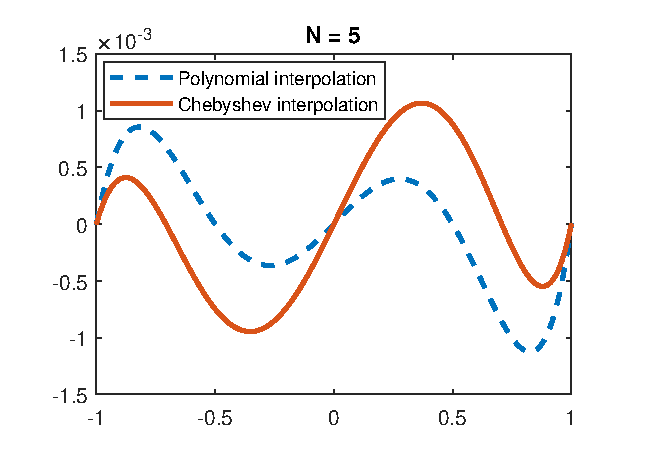
\includegraphics[width=3.2in]{./figs/e1a.eps}
      	\hspace{-6pt}
     	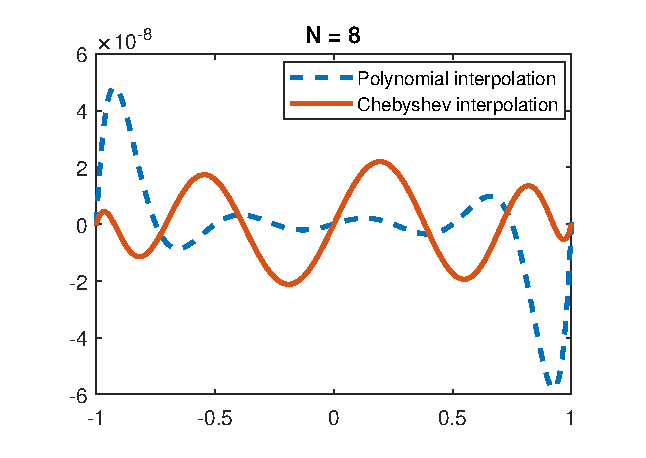
\includegraphics[width=3.2in]{./figs/e1b.eps}}
     	\hspace{-6pt}
		\caption{Errors of interpolations for the fucntion $e^x$ with points $N=4$ and $N=8$}
        \label{fig:e1}
\end{figure}
\end{exmp}

\begin{exmp}
In this example, we interpolate function $f(x)=1/(1+12x^2)$ by using both polynomial and chebyshev method with 15 points. Figure \eqref{fig:e2} shows Runge phenomenon from polynomial interpolation.\\
\begin{figure}     	\centerline{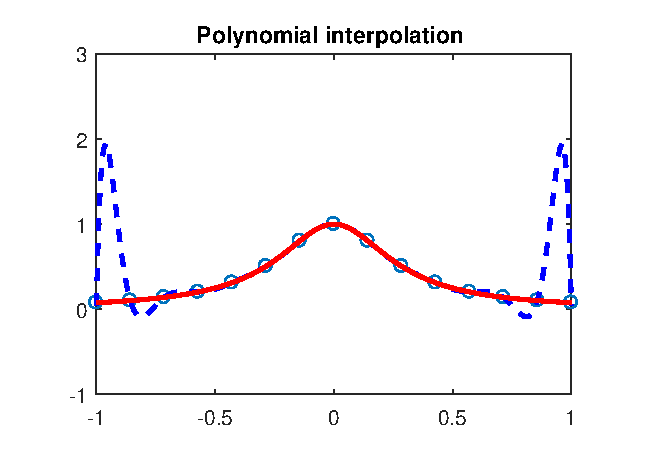
\includegraphics[width=3.2in]{./figs/e2a.eps}
      	\hspace{-6pt}
     	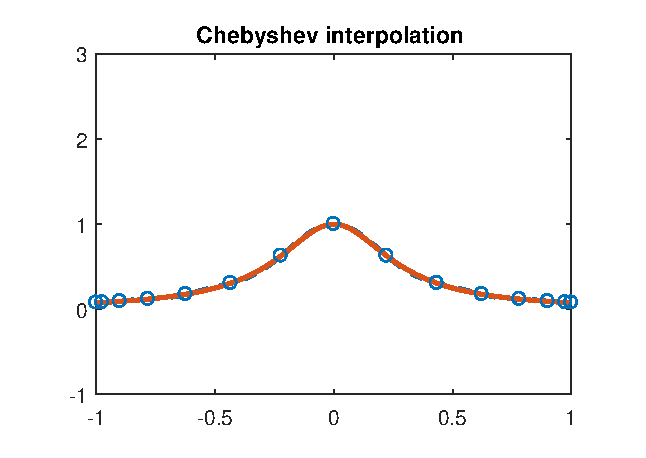
\includegraphics[width=3.2in]{./figs/e2b.eps}}
     	\hspace{-6pt}
		\caption{Interpolation of function $f(x)=\frac{1}{1+12x^2}$}
        \label{fig:e2}
\end{figure}
\end{exmp}

\section{Results and Discussions}
\section{acknowledgement}

\begin{thebibliography}{9}
\bibitem{Zachary}
  Zachary Battles and Lloyd N. Trefethen
  \emph{An Extension of Matlab to Continuous Function and Operations}.
  SIAM J. SCI. COMPUT Vol. 25, No. 5: 1743-1770 
  
\bibitem{CSG Operations}
Younis Hijazi, Aaron Knoll, Mathias Schott, Andrew Kensler, Charles Hansen and Hans Hagen
\emph{CSG Operations of Arbitrary Primitives with Interval Arithmetic and Real-Time Ray Casting}.
Scientific Visualization: Advanced Concepts, 78-89 (1998) 
	
\bibitem{Boolean Operations}
Yohan D. Fougerolle, Andrei Gribok, Sebti Foufou, Frederic Truchetet and Mongi A. Abidi
\emph{Boolean Operations with Implicit and Parametric Representation of Primitives Using R-Functions}.
IEEE Transactions on Visualization and Computer Graphics, Vol. 11, No. 5 (2005).
  
\bibitem{BRDF}
Chris Wynn
\emph{An Introduction to BRDF-Based Lighting}.
NVIDIA Corporation, 2000

\bibitem{CookTorr}
Robert Cook and Kenneth Torrance
\emph{A reflectance model for computer graphics. Computer Graphics}, Proc. of SIGGRAPH 81: 244-253 (1981).  
	
\bibitem{Ward}
Gregory J. Ward 
\emph{Measuring and Modeling Anisotropic Reflection. (SIGGRAPH 92),}: 265-272 (1992).

\bibitem{BlinnPhong}
James F. Blinn  
\emph{Models of light reflection for computer synthesized pictures}, Proc. 4th
Annual Conference on Computer Graphics and Interactive Techniques: 192-198
(1977). 

\end{thebibliography}

\bibliographystyle{plain}
%\bibliography{paper}

\end{document}
